\hypertarget{subsec:IndexToLevel}{}
\subsection{Implementing IndexToLevel}
\genHeader

If everything has been done correctly up to this point, your project should save and build (hit the hammer symbol in the eMolfon task bar).
The generated code will have some compilation errors (Step 1 in \Cref{eclipse:tggGenerated}) as Eclipse does not know where to access the generated code for the imported source and target ecore files (these could also be supplied from jars or installed plugins).
In our case the generated code is in the respective source and target projects so let's communicate this to Eclipse.

\begin{enumerate}

\item[$\blacktriangleright$] Open the \texttt{MANIFEST.MF} file (Step 2 in \Cref{eclipse:tggGenerated}) and choose the \texttt{De\-pen\-den\-cies} tab (Step 3).

\item[$\blacktriangleright$] Choose both source and target projects (Step 4) as dependencies and click \texttt{OK}.
All compilations errors should now be resolved.
\end{enumerate}

\begin{figure}[htb]
\begin{center}
  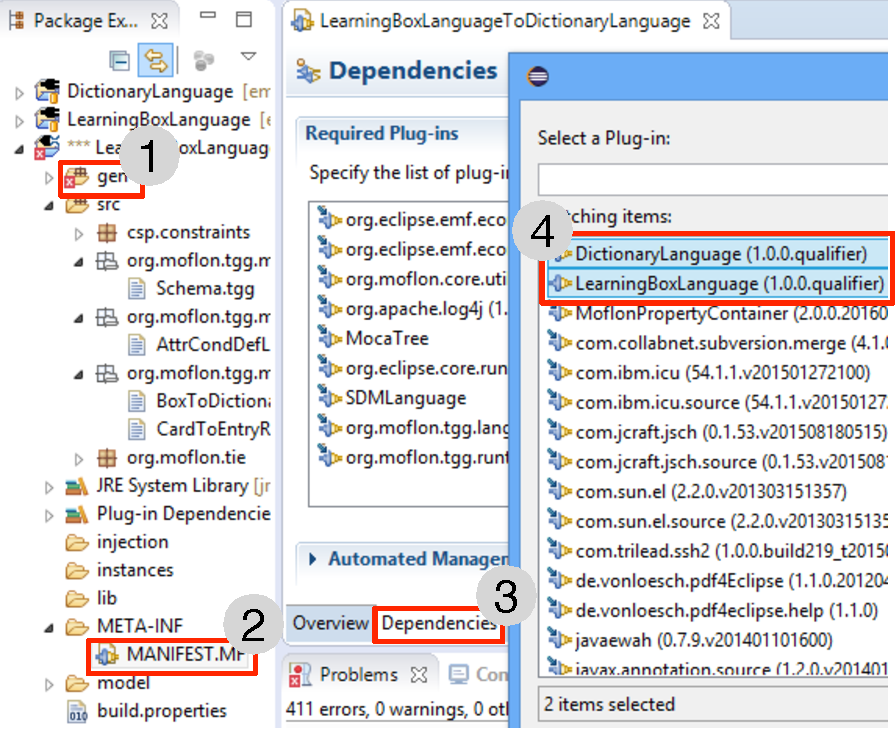
\includegraphics[width=0.8\textwidth]{eclipse_generatedTGG}
  \caption{Add source and target projects as dependencies}
  \label{eclipse:tggGenerated}
\end{center}
\end{figure}

Our TGG still isn't yet complete. 
While we've declared and actually used our custom \texttt{indexTolevel} attribute condition, we haven't actually implemented it yet. 
Let's quickly review the purpose of attribute conditions.

Just like patterns describing \emph{structural} correspondence, \emph{attribute conditions} can be automatically \emph{operationalized} as required, e.g., for a forward transformations. 
Even more interesting, a set of attribute conditions might have to be ordered in a specific way depending on the direction of the transformation.
Enforcing the conditions might involve checking existing attribute values, or setting these values appropriately.

For built-in \emph{library} attribute conditions such as \emph{eq}, \emph{addPrefix} and \emph{concat}, you do not need to worry about these details and can just focus
on expressing what should hold. 
Everything else is handled automatically.

In some cases however, a required attribute condition might be problem-specific, such as our \emph{indexToLevel}. 
There might not be any fitting combination of library attribute conditions to express the consistency condition, so a new attribute condition type must be declared and implemented.

There is a list of \emph{adornments} in the declaration which specify the cases for which the attribute condition can be operationalized. 
Each adornment consists of a \texttt{B} (bound) or \texttt{F} (free) variable setting for each argument of the attribute condition. 
This might sound a bit complex, but it's really quite simple, especially in the context of our example:

\begin{description}

\item[BB] indicates that the \texttt{partition.index} and \texttt{entry.level} are both \emph{bound}, i.e., they already have assigned values.
In this case, the \emph{operation} must check if the assigned values are valid and correct.

\item[BF] indicates that \texttt{partition.index} is \emph{bound} and \texttt{entry.level} is \emph{free}, i.e., the operation must determine and assign the correct value to \texttt{entry.level} using \texttt{partition.index}.

\item[FB] would indicate that \texttt{partition.index} is \emph{free} and \texttt{entry.level} is \emph{bound}, i.e., the operation must determine and assign the correct value to \texttt{parti\-tion.in\-dex} using \texttt{entry.level}.

\item[FF] would indicate that both \texttt{partition.index} and \texttt{entry.level} are \emph{free} and we have to somehow generate consistent values out of thin air.

\end{description}

As \texttt{partition} is a context element in the rule (the partition is always bound in whatever direction), \textbf{FF} and \textbf{FB} are irrelevant cases and we do not need to declare or implement what they mean.
For the record, note that adornments can be declared as either \texttt{\#gen} or \texttt{\#sync}.
The reason is that it might make sense to restrict some adornments (typically \textbf{FF} cases) to only when generating models.
Using \textbf{FF} cases for synchronisation might possibly makes sense, but most of the time it would be weird to generate random values during a forward or backward synchronisation.  

At compile time, the set of attribute conditions for every TGG rule is ``solved'' for each case by
operationalizing all constraints and determining a feasible sequence in which the operations can be executed, compatible to the declared adornments of each attribute condition. 
If the set of attribute conditions cannot be solved, an exception is thrown at compile time.

Now that we have a better understanding behind the construction of attribute conditions, let's implement \texttt{indexToLevel}.

\begin{itemize}
\item[$\blacktriangleright$] Locate and open \texttt{IndexToLevel.java} under ``src/csp.constraints'' in \texttt{LearningBoxToDictionaryIntegration}.

\item[$\blacktriangleright$] As you can see, some code has been generated in order to handle the current unimplemented state of \texttt{IndexToLevel}. 
Use the code depicted in \Cref{code:indexToLevel} to replace this default implementation.\footnote{Depending of course on your pdf viewer, copy and pasting this code should work.}

\begin{figure}[htb]
\begin{verbatim}
package csp.constraints;

import java.util.Arrays;
import java.util.List;
import org.moflon.tgg.language.csp.Variable;
import org.moflon.tgg.language.csp.impl.TGGConstraintImpl;

public class IndexToLevel extends TGGConstraintImpl {

    private static List<String> levels = 
      Arrays.asList(new String[] {"master","advanced","beginner"});

    public void solve(Variable var_0, Variable var_1) {
        int index = ((Integer) var_0.getValue()).intValue();
        int normalisedIndex = Math.min(Math.max(0, index), 2);
        String bindingStates = getBindingStates(var_0, var_1);
        
        switch (bindingStates) {
        case "BB":
            String level = (String) var_1.getValue();
            setSatisfied(levels.get(normalisedIndex).equals(level));
            break;
        case "BF":
            var_1.bindToValue(levels.get(normalisedIndex));
            setSatisfied(true);
            break;
        }}}
\end{verbatim}
  \caption{Implementation of our custom \texttt{IndexToLevel} constraint}
  \label{code:indexToLevel}
\end{figure}

\end{itemize}

To briefly explain, the \texttt{levels} list contains difficulty level at positions 0, 1, or 2 in the list, which correspond to our three partitions in the learning box. 
You'll notice that instead of setting ``master'' to 2, it has rather been set to match the first 0th partition. 
Unlike an \texttt{entry} in \texttt{dictionary}, the position of each \texttt{card} in \texttt{box} is \emph{not} based on difficulty, but simply how it has been moved as a result of the user's correct and incorrect guesses. 
Easy cards are more likely to be in the final partition (due to moving through the box quickly) while challenging cards are most likely to have been returned to (and currently to be at) the starting position, i.e., the 0th partition.

In the \texttt{solve} method, the index of the matched partition in the rule is first of all normalised (negative values do not make sense, and we handle all partitions  after partition 2 in the same way).
A switch statement is then used, based on whichever adornment is currently the case, to enforce or check the condition. 

For \texttt{BB} we check if the normalised index of the partition corresponds to the difficulty level of the card.
For \texttt{BF}, the normalised index is used to set the appropriate difficulty level of the card.

%%% Local Variables: 
%%% mode: latex
%%% TeX-master: "../src/TGG_mainFile"
%%% End: 
